\section{Sicherheit}
\label{sec:sicherheit_basics}

Wie aus der Abbildung in Abschnitt \ref{subsec:overlay_netzwerke} \textit{\nameref{subsec:overlay_netzwerke}} ersichtlich ist, ist das Overlay-Netzwerk die oberste Schicht des Peer-to-Peer-Netzwerks. Es sorgt dafür, dass sich die Teilnehmer des Netzwerks finden können. Die eigentliche Kommunikation, also das Senden und Empfangen von Nachrichten, erfolgt jedoch über das Internet. Da das Internet ein öffentliches Netzwerk ist, besteht die Gefahr, dass die Nachrichten abgefangen und mitgelesen werden können. Die Nachrichten müssen über Verteilerknoten oder Access Points übertragen werden, die nicht vertrauenswürdig sind. Um ein Mitlesen oder Verändern der Nachrichten zu verhindern, muss die Kommunikation abgesichert werden. 

Mittels Kryptografie kann die Vertraulichkeit, Integrität und Authentizität der Kommunikation gewährleistet werden \Parencite[S. 7]{Hellmann_IT-Sicherheit}.


\subsection{Vertraulichkeit}
\label{subsec:vertraulichkeit_basics}

Die Vertraulichkeit der Kommunikation wird durch Verschlüsselung gewährleistet. Man unterschiedet zwei Formen der Kryptografie: \textit{symmetrische} und \textit{asymmetrische} Kryptografie. Bei der \textit{symmetrischen} Kryptografie wird ein und derselbe Schlüssel zum Verschlüsseln und Entschlüsseln der Nachricht verwendet. Der Sender der Nachricht verschlüsselt die Nachricht mit einem Schlüssel und sendet die nun verschlüsselte Nachricht an den Empfänger. Der Empfänger kann die Nachricht mit dem gleichen Schlüssel entschlüsseln. Dadurch kann ein Angreifer, der die Nachricht abfängt, diese nicht entschlüsseln, da er den Schlüssel nicht kennt. Abbildung \ref{fig:symmetrische_verschluesselung} zeigt den Ablauf der symmetrischen Verschlüsselung.

\begin{center}
    \captionsetup{type=figure}
    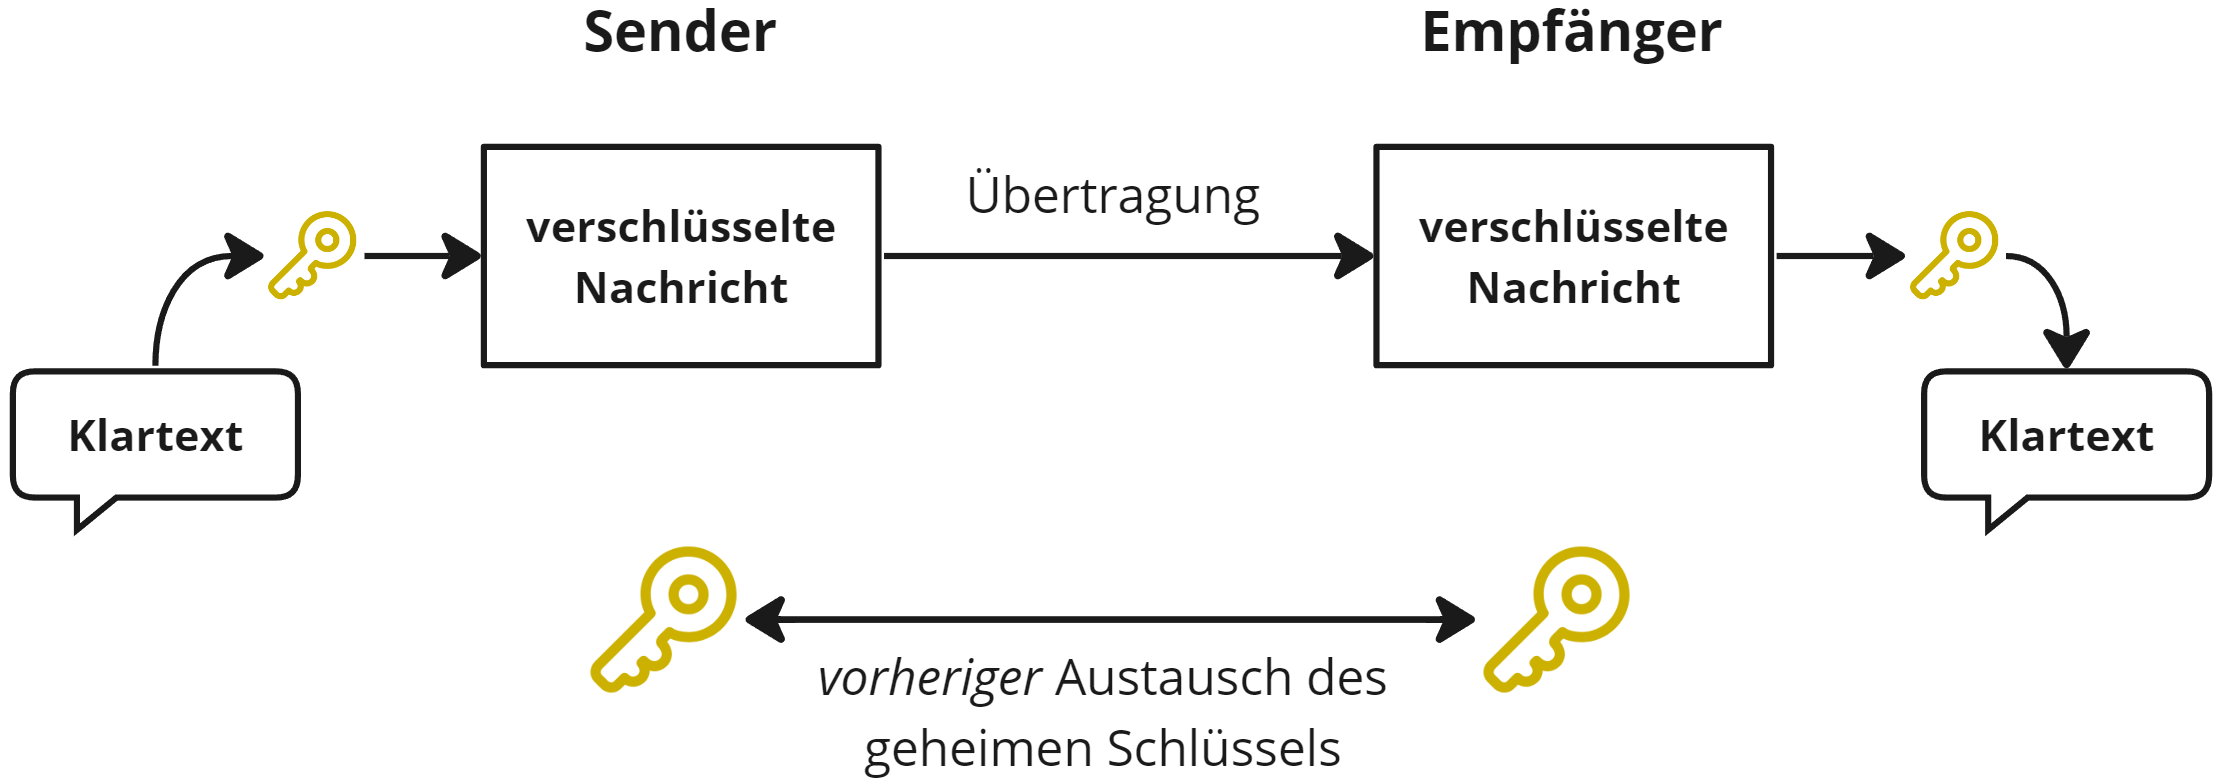
\includegraphics[width=1\linewidth]{images/symmetric_encryption.png}
    \caption{Symmetrische Verschlüsselung (in Anlehnung an \cite{ElektronikKompendium_symmetrischeVerschluesselung})}
    \label{fig:symmetrische_verschluesselung}
\end{center}

\noindent Das Problem bei der symmetrischen Kryptografie ist, dass der Schlüssel zu Beginn der Kommunikation vom Sender an den Empfänger gelangen muss. Dies stellt eine Herausforderung dar, wenn Sender und Empfänger sich noch nicht kennen und noch nie zuvor miteinander kommuniziert haben oder noch nicht über andere Wege einen Schlüssel ausgetauscht haben. Sollte der Schlüssel bei der Übertragung über einen unsicheren Kanal abgefangen werden, kann der Angreifer die Kommunikation entschlüsseln und somit mitlesen \Parencites[S. 644]{DiffieHellman_NewDirectionsInCryptography}[S. 5-8]{Wong_KryptoPraxis}. 

In diesem Fall kann eine Schlüsselvereinbarung verwendet werden, um einen gemeinsamen Schlüssel zu erhalten. Bei der Schlüsselvereinbarung wird ein Schlüssel zwischen zwei Parteien vereinbart, ohne dass dieser über einen unsicheren Kanal übertragen werden muss \Parencite[S. 102]{Wong_KryptoPraxis}. Abbildung \ref{fig:schluesselvereinbarung} zeigt den Ablauf der Schlüsselvereinbarung.

\begin{center}
    \captionsetup{type=figure}
    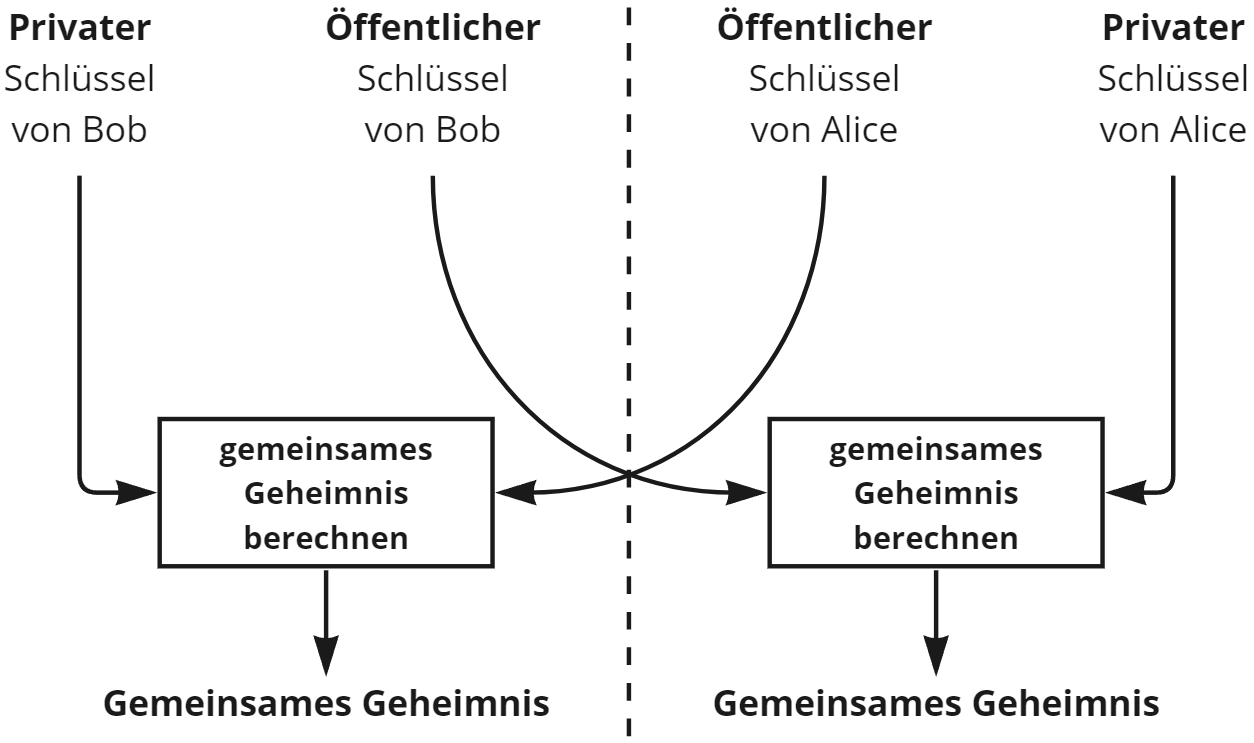
\includegraphics[width=0.7\linewidth]{images/key_exchange.png}
    \caption{Schlüsselvereinbarung (in Anlehnung an \cite[S. 102]{Wong_KryptoPraxis})}
    \label{fig:schluesselvereinbarung}
\end{center}

\noindent Beide Teilnehmer generieren einen privaten Schlüssel und einen öffentlichen Schlüssel. Durch die Kombination des öffentlichen Schlüssels des anderen Teilnehmers und des eigenen privaten Schlüssels wird ein gemeinsames Geheimnis berechnet. Dieses gemeinsame Geheimnis kann dann für die symmetrische Verschlüsselung verwendet werden, da dadurch beide Teilnehmer den gleichen Schlüssel besitzen \Parencite[S. 102]{Wong_KryptoPraxis}.


Bei der \textit{asymmetrische} Kryptografie (auch \textit{Public-Key-Kryptografie} genannt) wird anstatt nur eines Schlüssels ein Schlüsselpaar generiert, das aus einem öffentlichen und einem privaten Schlüssel besteht. Der öffentliche Schlüssel des Empfängers wird zum Verschlüsseln der Nachrichten verwendet und zum Entschlüsseln der Nachrichten wird der private Schlüssel des Empfängers verwendet. Der öffentliche Schlüssel des Empfängers kann von jedem verwendet werden, um Nachrichten an den Empfänger zu verschlüsseln. Nur der Empfänger kann die Nachrichten entschlüsseln, da nur er den privaten Schlüssel besitzt. Der Ablauf der asymmetrischen Verschlüsselung ist in Abbildung \ref{fig:asymmetrische_verschluesselung} dargestellt.


\begin{center}
    \captionsetup{type=figure}
    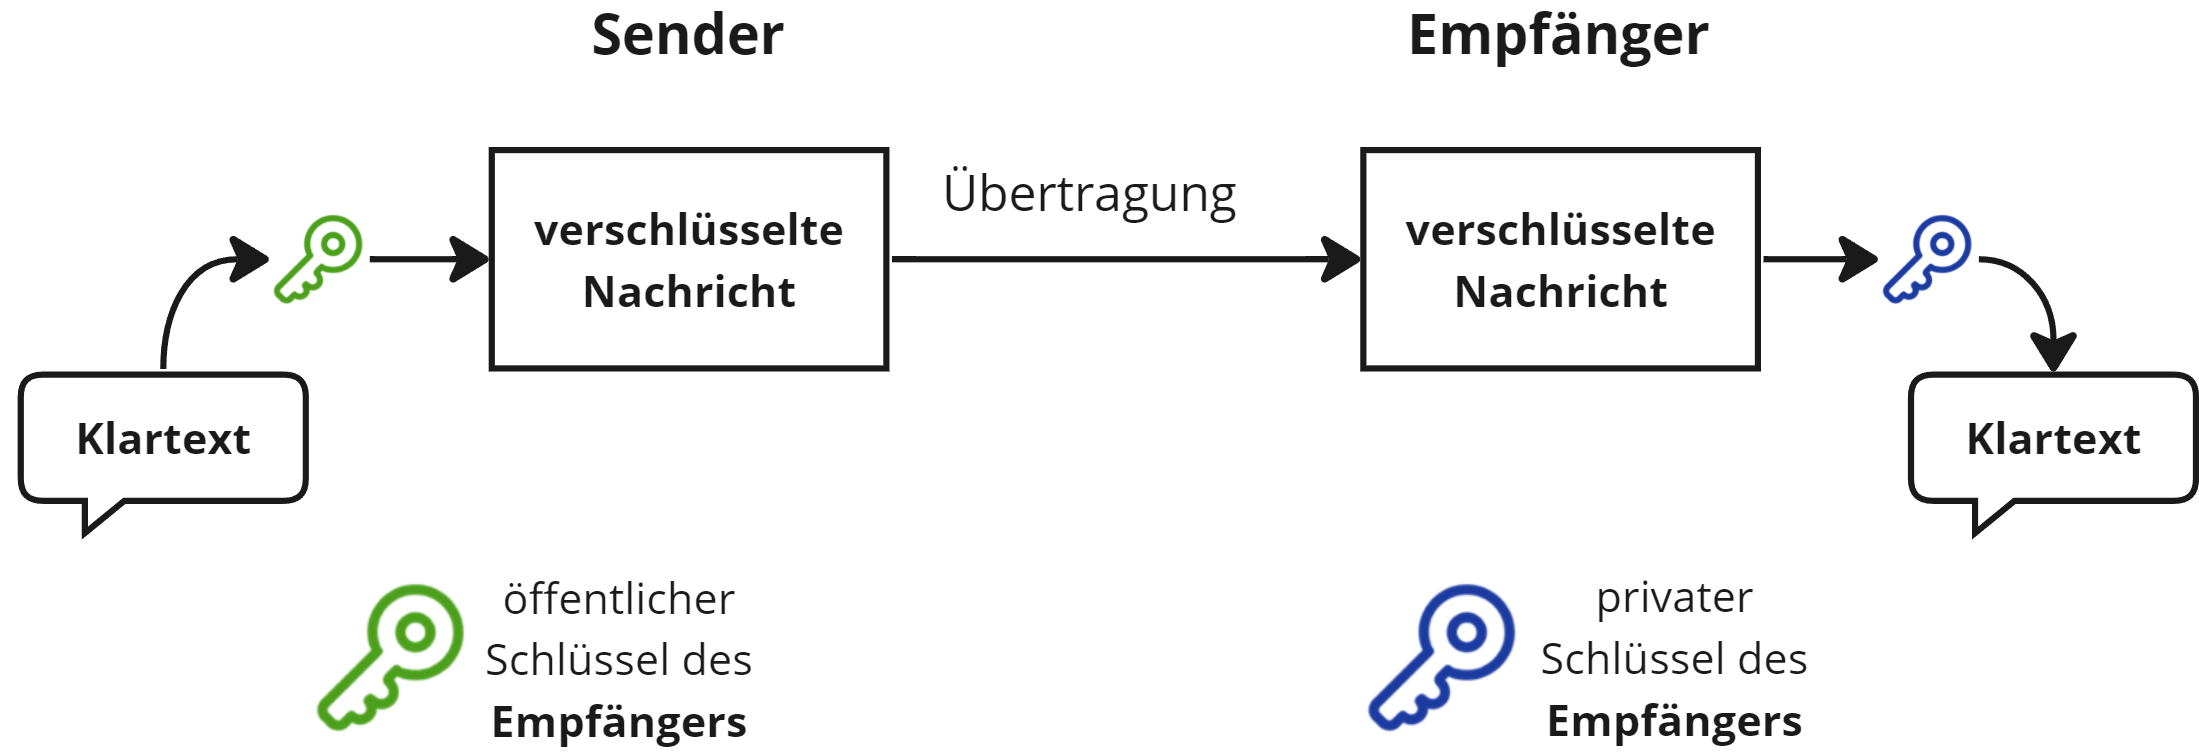
\includegraphics[width=1\linewidth]{images/asymmetric_encryption.png}
    \caption{Asymmetrische Verschlüsselung (in Anlehnung an \cite{ElektronikKompendium_asymmetrischeVerschluesselung})}
    \label{fig:asymmetrische_verschluesselung}
\end{center}

\noindent Es ist außerdem nicht möglich, Nachrichten, die mit dem öffentlichen Schlüssel verschlüsselt wurden, mit diesem auch wieder zu entschlüsseln \parencite{ElektronikKompendium_asymmetrischeVerschluesselung}. 

Diese kryptografische Verfahren können kombiniert werden, um die Vorteile von diesen zu nutzen. Der Schlüsselaustausch wird mit der asymmetrischen Verschlüsselung durchgeführt und die eigentliche Kommunikation wird mit der symmetrischen Verschlüsselung durchgeführt.


\subsection{Integrität}
\label{subsec:integritaet_signatur}

Um die Integrität der Kommunikation zu gewährleisten, wird Hashing verwendet. Das Hashing von Daten erfordert die Verwendung einer \textit{Hash-Funktion}. Hash-Funktionen sind Funktionen, die eine Eingabe beliebiger Länge in eine Ausgabe fester Länge umwandeln. Dabei ist es wichtig, dass die Hash-Funktion zwei Eigenschaften erfüllt: \textit{Einwegfunktion} und \textit{Kollisionsresistenz}. Eine Hash-Funktion erfüllt die Eigenschaft der Einwegfunktion, wenn es nicht möglich ist, von der Ausgabe auf die Eingabe zu schließen. Das bedeutet, dass es nicht möglich ist, aus dem Hash-Wert die ursprünglichen Daten zu rekonstruieren. Die Eigenschaft der Kollisionsresistenz ist erfüllt, wenn es nicht möglich ist, zwei verschiedene Eingaben zu finden, die auf den gleichen Hash-Wert abgebildet werden \parencites[S. 12-13]{Brünnler_BlockchainKurzGut}[S. 6]{Fill_BlockchainGrundlagen}.

Das Ergebnis der Hash-Funktion ist eine Zeichenkette, die aus einer festen Anzahl an Zeichen besteht und als \textit{Hash-Wert} oder auch nur \textit{Hash} bezeichnet wird. Der Hash-Wert ist ein eindeutiger Fingerabdruck der Daten, die in die Hash-Funktion eingegeben wurden. Sollte sich also der Inhalt der Daten ändern, ändert sich auch der Hash-Wert. 


\subsection{Authentizität}

In Kombination mit einer sogenannten Signatur kann zusätzlich zur Integrität auch die Authentizität einer Nachricht gewährleistet werden. Abbildung \ref{fig:signatur} zeigt, wie eine Nachricht digital signiert wird.

\begin{center}
    \captionsetup{type=figure}
    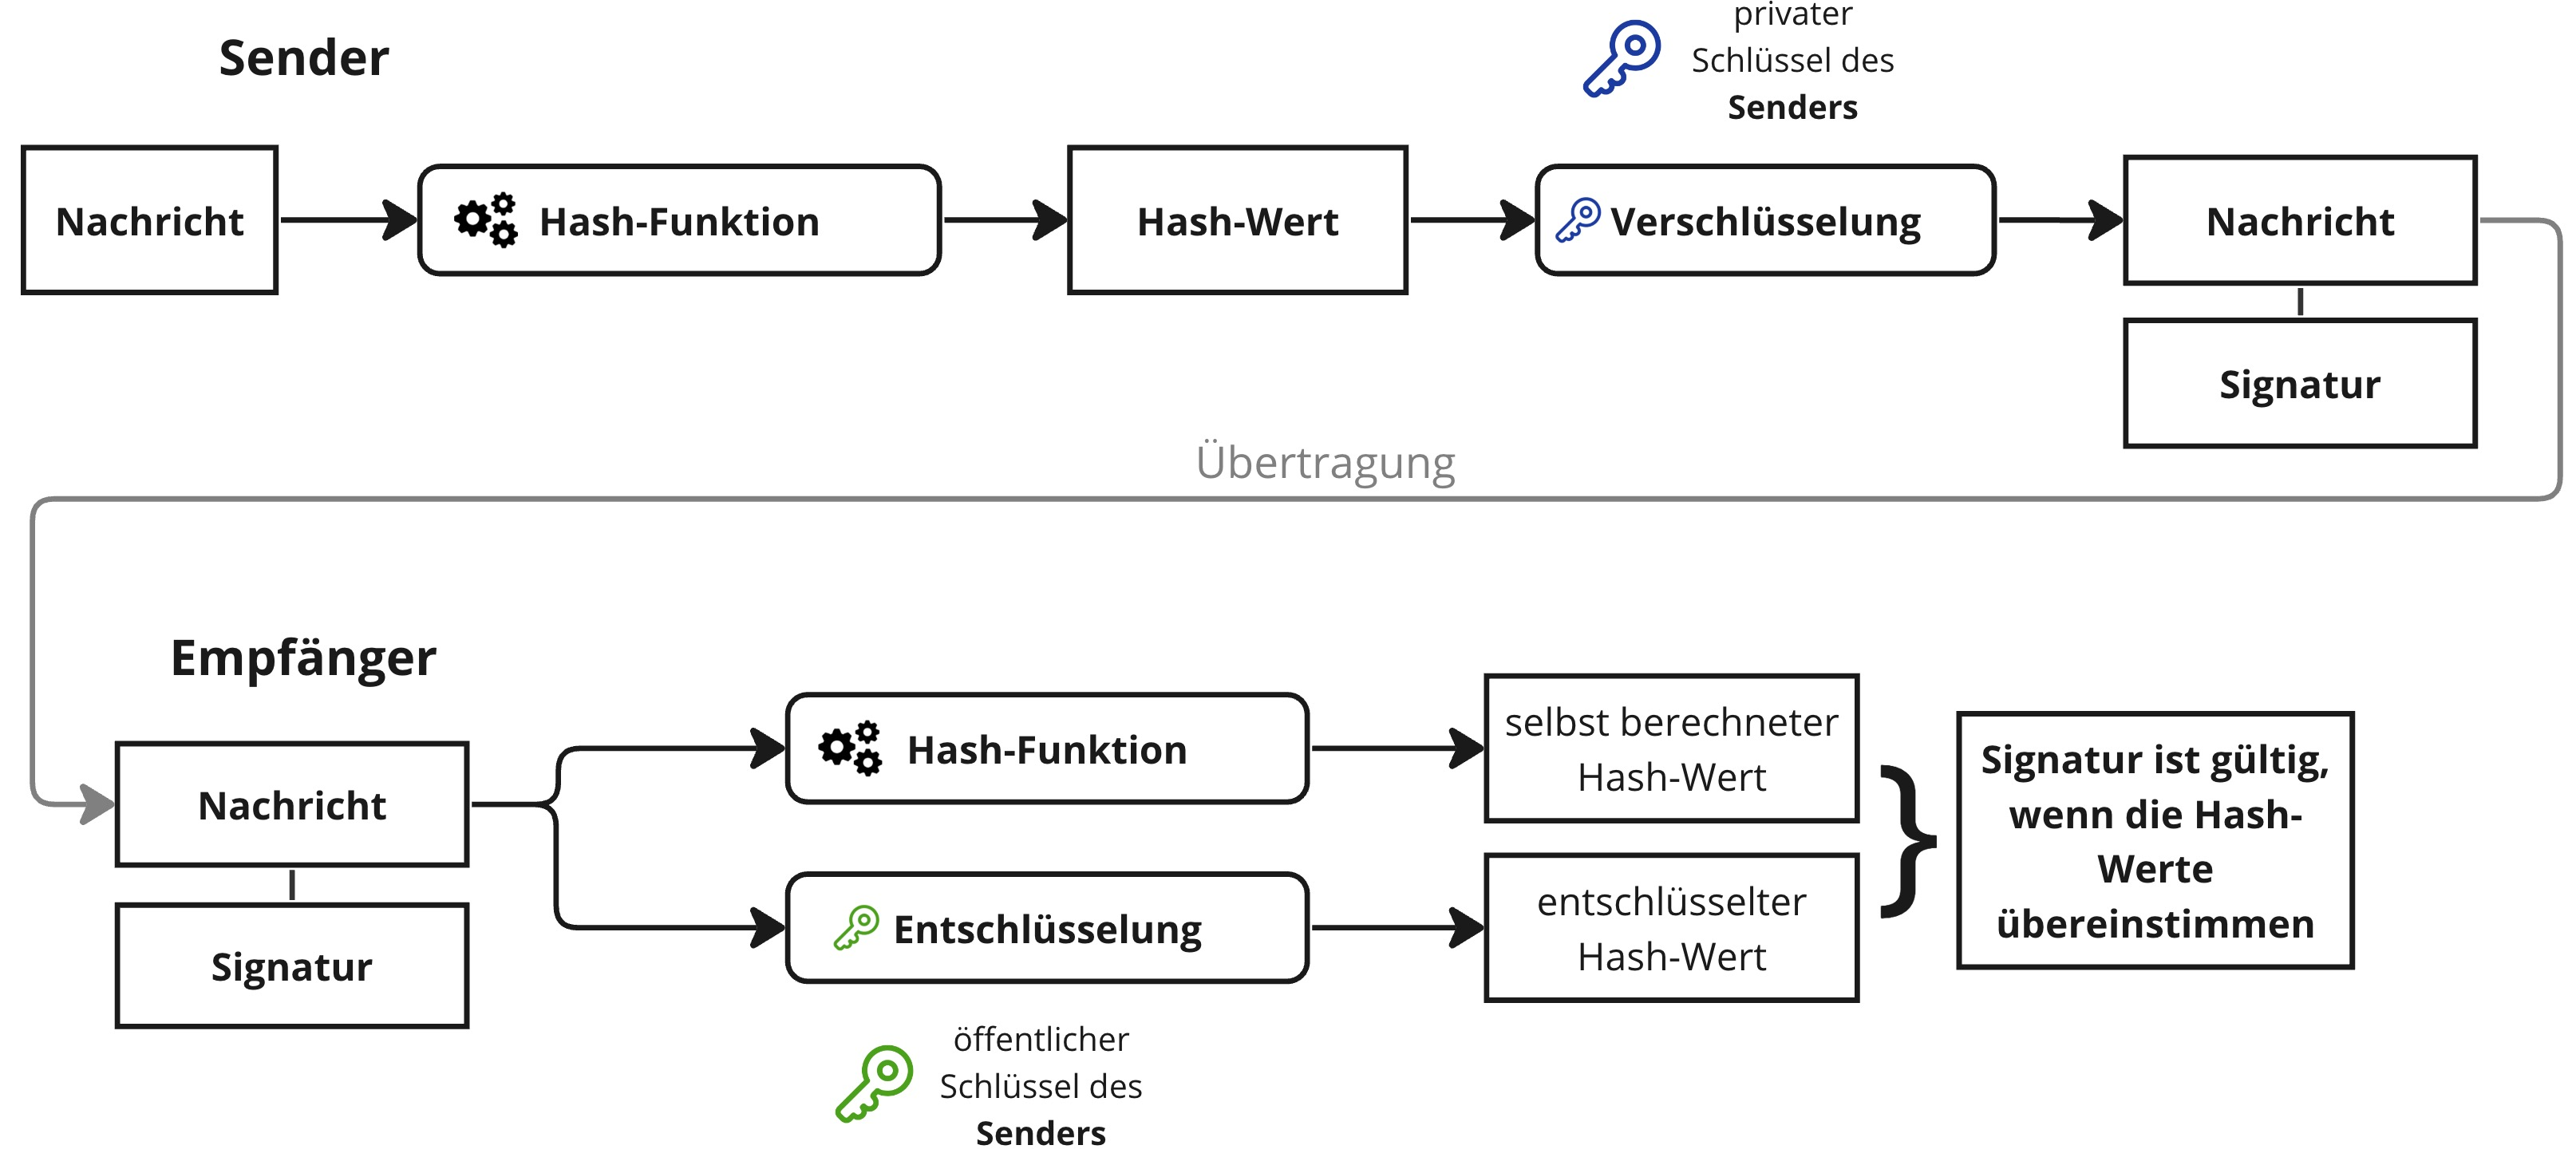
\includegraphics[width=1\linewidth]{images/signatur_2.jpg}
    \caption{Signieren einer Nachricht (in Anlehnung an \cite{DocuSign_digitaleSignaturen})}
    \label{fig:signatur}
\end{center}


\noindent Der Sender berechnet den Hash-Wert der Nachricht, verschlüsselt diesen mit seinem privaten Schlüssel. Das Ergebnis ist die digitale Signatur, welche an die Nachricht angehängt wird. Der Empfänger braucht den öffentlichen Schlüssel des Senders, um die Signatur zu entschlüsseln. Dafür gibt es verschiedene Möglichkeiten. Eine Möglichkeit ist, dass der Sender den öffentlichen Schlüssel dem Empfänger vorher über einen sicheren Kanal übermittelt. Eine andere Möglichkeit ist, dass der öffentliche Schlüssel des Senders in einem öffentlichen Schlüsselverzeichnis gespeichert ist. Wenn der Empfänger den öffentlichen Schlüssel des Senders besitzt, kann er die Signatur entschlüsseln. Gleichzeitig berechnet der Empfänger den Hash-Wert der Nachricht. Wenn der berechnete Hash-Wert mit dem entschlüsselten Hash-Wert übereinstimmt, kann der Empfänger einerseits sicher sein, dass die Nachricht nicht verändert wurde und somit die Integrität der Nachricht gewährleistet ist und andererseits, dass die Nachricht vom Sender stammt und somit die Authentizität der Nachricht gewährleistet ist. Falls der berechnete Hash-Wert nicht mit dem entschlüsselten Hash-Wert übereinstimmt, wurde die Nachricht entweder verändert oder die Nachricht stammt nicht vom erwarteten Sender \Parencite[S. 73-78]{Hellmann_IT-Sicherheit}.


\subsection{Ende-zu-Ende-Verschlüsselung}
\label{subsec:signal_protokoll_basics}

% Was ist Ende-zu-Ende-Verschlüsselung? Wie entsteht diese? Warum zeige ich das anhand des Signal-Protokolls?

Die behandelten Sicherheitsmechanismen können zu einer sogenannten Ende-zu-Ende-Verschlüsselung kombiniert werden. Diese erlaubt es, dass nur der Sender und der Empfänger die Nachrichten lesen können. Eine moderne Variante der Ende-zu-Ende-Verschlüs-\\selung ist das Signal-Protokoll. Dies wird auch in der Signal-App verwendet (\ref{subsubsection:signal} \textit{\nameref{subsubsection:signal}}). Im Folgenden wird das Signal-Protokoll genauer beschrieben.

Zu Beginn einer Sitzung wird ein gemeinsamer Schlüssel zwischen den Teilnehmern vereinbart. Das Signal-Protokoll verwendet hierfür ein spezielles Verfahren, das sich \textit{Extended Triple Diffie-Hellman} oder auch kurz \textit{X3DH} nennt. Dieses kombiniert mehrere Schlüsselaustauschaktionen, und ist dadurch in der Lage, einen gemeinsamen Schlüssel zu berechnen, ohne dass der Kommunikationspartner direkt erreichbar sein muss. Dazu werden mehrere flüchtige Schlüssel auf einem Server gespeichert. Dies dient dazu, dass eine Kompromittierung dieser Schlüssel nicht die Sicherheit der Kommunikation gefährdet, da diese nur für eine begrenzte Zeit gültig sind und für jede Sitzung neu generiert werden \Parencite[S. 249-252]{Wong_KryptoPraxis}.


Da solch eine Sitzung sehr lange dauern kann, generiert das Signal-Protokoll auch für jede Nachricht einen neuen Schlüssel. Hierfür wird der sogenannte \textit{Double Ratchet Algorithmus} verwendet. Dieser bildet den Kern des Signal-Protokolls. Eine \textit{Ratchet} (zu Deutsch: \textit{Ratsche}) ist ein Werkzeug, das nur in eine Richtung gedreht werden kann. Diese Eigenschaft wird auf die verwendeten Schlüssel angewendet. Dadurch ist es nicht möglich, vorherige Schlüssel zu berechnen, was auch als \textit{Forward Secrecy} bezeichnet wird. Der Algorithmus verwendet zwei Ratchet-Schritte. Der erste Ratchet-Schritt verwendet einen symmetrischen Schlüssel. Basierend auf dem vorher, durch X3DH vereinbarten, gemeinsamen Schlüssel, generieren die Kommunikationspartner jeweils einen Empfangs- und einen Sendeschlüssel. Jede gesendete Nachricht wird dem Sendeschlüssel verschlüsselt und jede empfangene Nachricht wird mit dem Empfangsschlüssel entschlüsselt. Nach jeder Nachricht werden die Schlüssel durch eine Schlüsselableitungsfunktion aktualisiert. Der zweite Ratchet-Schritt ist ein asymmetrischer Schlüsselaustausch, den die Kommunikationspartner periodisch austauschen \Parencite[S. 252-257]{Wong_KryptoPraxis}. 

Vereinfacht kann der Double Ratchet Algorithmus für einen der Kommunikationspartner folgendermaßen dargestellt werden (siehe Abbildung \ref{fig:double_ratchet}):


\begin{center}
    \captionsetup{type=figure}
    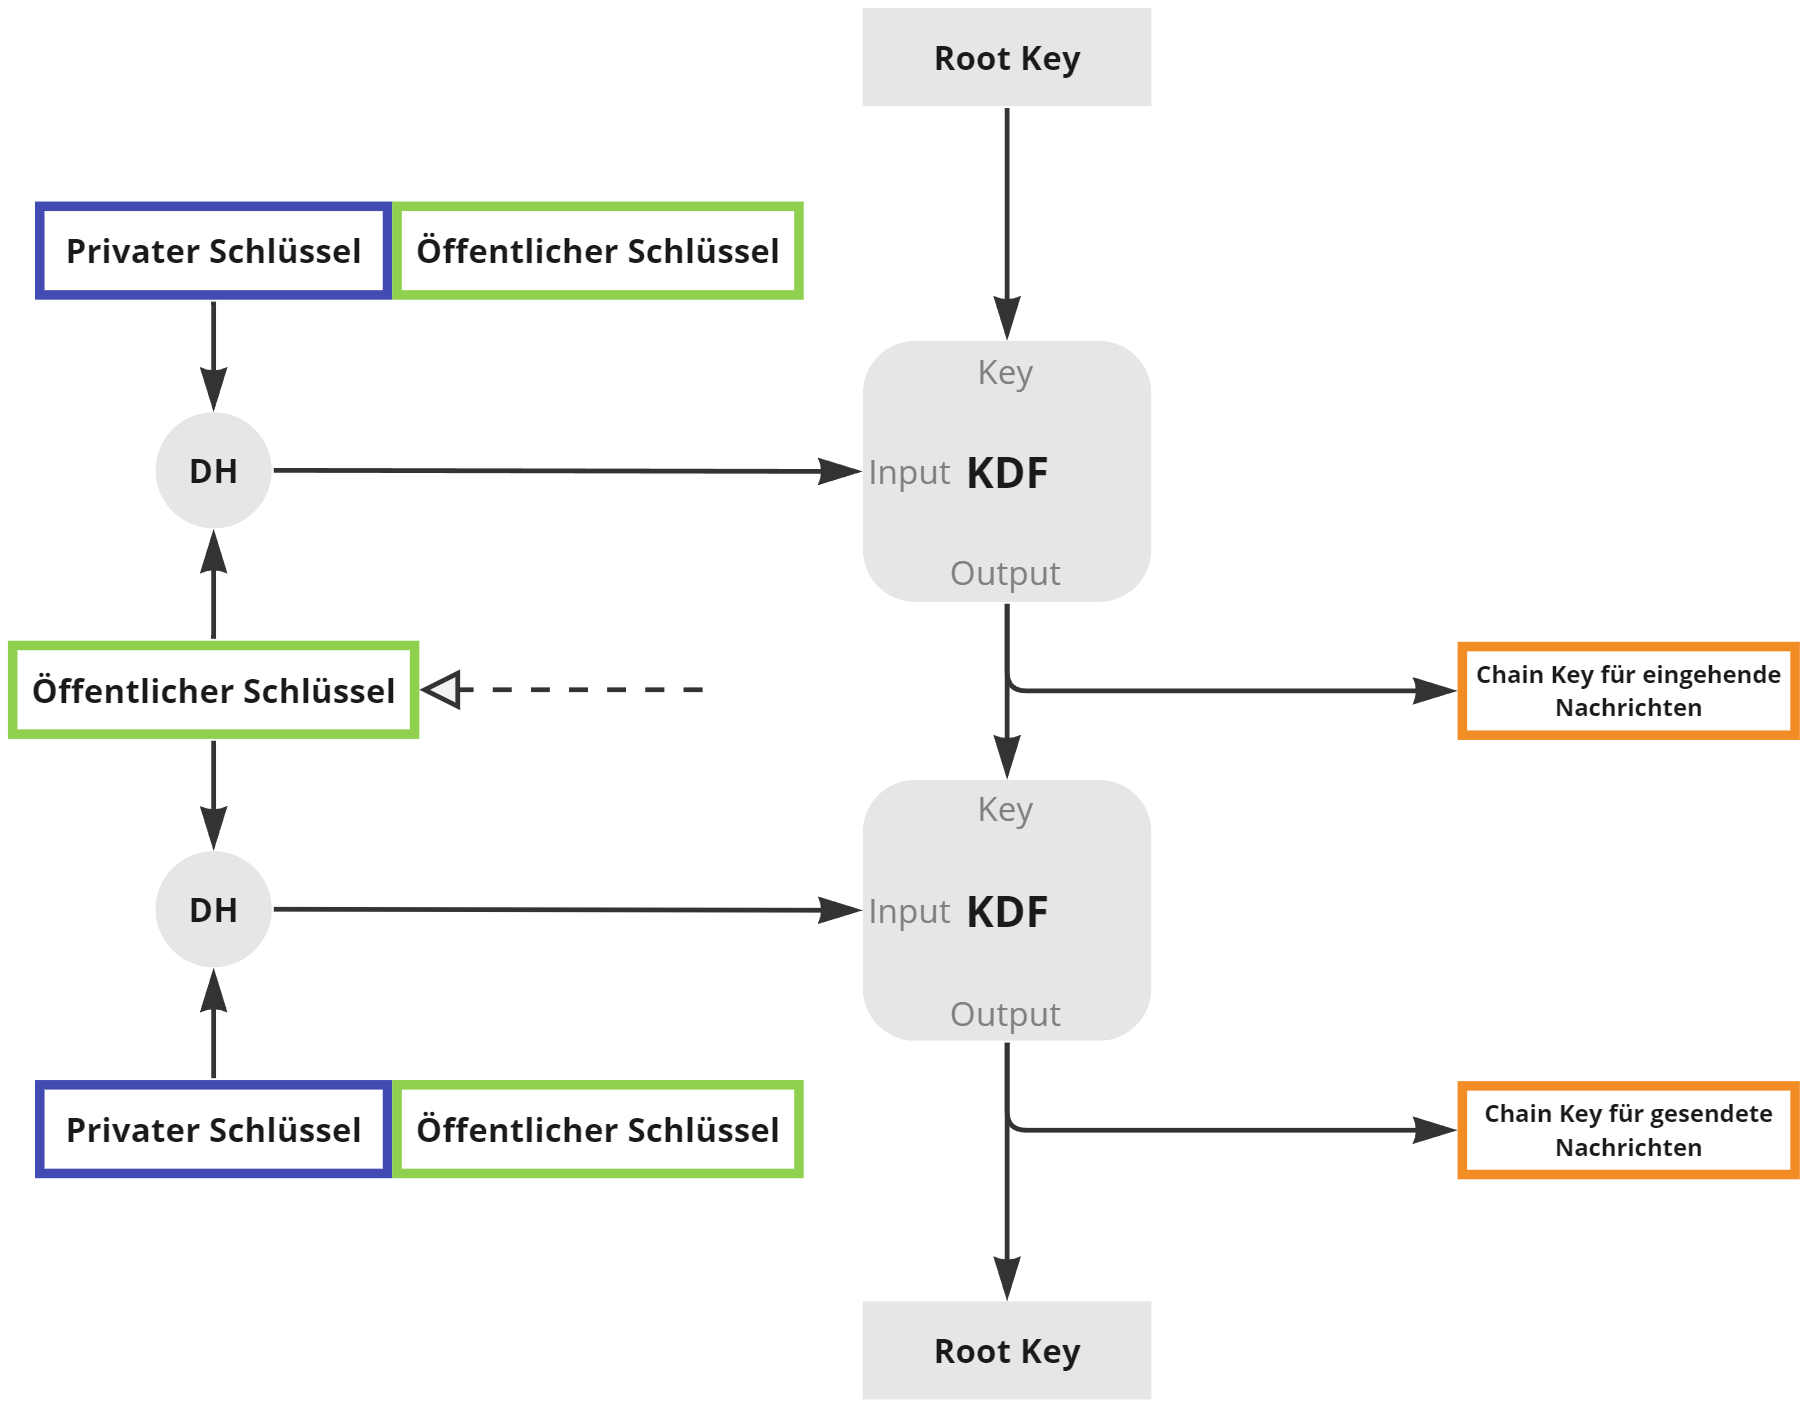
\includegraphics[width=0.8\linewidth]{images/double_ratchet_altered.png}
    \caption{Vereinfachter Double Ratchet Algorithmus (in Anlehnung an \cite{Signal_DoubleRatchet})}
    \label{fig:double_ratchet}
\end{center}

\noindent Links ist der zweite Ratchet-Schritt zu sehen (asymmetrischer Schlüsselaustausch). In der Abbildung ist dieser mit \textit{DH} gekennzeichnet, was für den Diffie-Hellman-Schlüsselaus-\\tausch steht. Auf der rechten Seite befindet sich der erste Ratchet-Schritt. Die Schlüsselableitungsfunktion wird in der Abbildung mit \textit{KDF} bezeichnet. Aus dieser werden die symmetrischen Schlüssel (in der Abbildung als \textit{Chain Key} bezeichnet) abgeleitet, die die jeweiligen Nachrichten ver- und entschlüsseln.

